\section{The {\tt WHILE} Language\timeestimation{15h}}
\label{sec:WHILE}
While most modern programming languages today are turing complete and as such
are "equally powerful". For simplicity however not all languages are created
equal, as section \ref{sec:Turing Completeness} will note. Lets therefore
introduce a simple, but expressive enough language called {\tt WHILE}.

\begin{table*}[h]
	\begin{align*}
		Expression \ni E, F::= \qquad
										& \mathtt{nil} & | \\
										& \mathtt{cons}\; E\; F & | \\
										& \mathtt{hd}\; E     & | \\
										& \mathtt{tl}\; E     & | \\
										& \mathtt{[}I \mathtt{](} E \mathtt{)}      & | \\
										& I \\
		Statement \ni S, T::= \qquad
										& I \mathtt{:=} E & | \\
										& \mathtt{while}\; E\; \mathtt{\{}\; S\; \mathtt{\}} & | \\
										& S \; \text{\tt{<newline>}}\; T \\
		Program \ni P, Q::= \qquad
										& I_1\; \mathtt{read}\; I_2\; \mathtt{\{}\; S\; \mathtt{\}}\; \mathtt{write}\; I_3 & | \\
										& Q  \; \text{\tt{<newline>}}\; P
	\end{align*}
\end{table*}

\subsection{The Elements} % (fold)
\label{sub:The Elements}
The {\tt WHILE} language contains only very basic commands, but they can be combined
to implement any algorithm (up to coding). As we will see, we only need a data
structure that is not bounded in its range (something for example {\tt int}s in
Java fail to be). An expression is then something, that can be evaluated to
such an data structure. For the purposes of this text, the {\tt cons} cell data
structure will be used, a cell that contains only a head and a tail (an
observant reader will notice that this structure stems from the building of
linked lists). 

\begin{figure}[htb]
	\begin{center}
		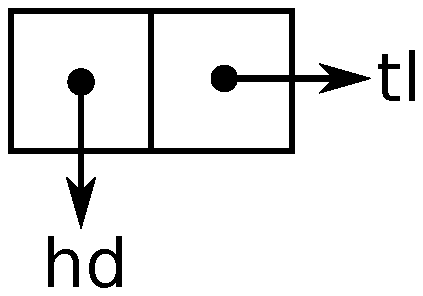
\includegraphics[height=3cm]{while/images/conscell}
	\end{center}
	\caption{The {\tt cons} cell}
\end{figure}

In while the call {\tt cons e1 e2}, where e1 and e2 are again
expressions, constructs such a cell with the value of e1 in the head and the
value of e2 in the tail. The expression "hd e1" yields the head of the value of
e1 and "tl e1" the tail. since all our current constructs need another
expression, we also need a "bottom" to this regress. We add nil as an
expression, which is distinct from any "cons e f". We also want to refer to
stored values, so an identifier (eg X) can also be an expression. 

Then there are statements. Statements change something about the state of the
program. In the case of while, there is only the assignment as an atomic
statement, which contains an identifier on the left side of an ":=" and an
expression on the right side. The other important statement is the WHILE
statement, which takes an data expression and a block of statements and as long
as the expression does not evaluate to nil, the block is executed. 

Finally there are procedures. Procedures read an input and write an output and
execute some statements in between. (picture of input: data, black box, output:
data)

Procedures can be called by their names in brackets and the argument (a data
expression). Now however that this is just a convenience, so as to make writing
a moderately simple WHILE programs possible. One could just write everything
out, but that would be cumbersome and not very helpful in understanding
computability or complexity.

% subsection The Elements (end)
\paragraph{Alternatives to the {\tt WHILE} construct} % (fold)
\label{par:Alternatives to the WHILE construct}
\lineofthought{
	\begin{itemize}
		\item Unrestricted Recursion
		\item Unbound Search ($\mu$)
		\item Applying transition rules as long as possible (Markov)
  \end{itemize}
}
% paragraph Alternatives to the WHILE construct (end)
\subsubsection{Natural Numbers} % (fold)
\label{ssub:Natural Numbers}
\lineofthought{Bei \cite{jones} sind Zahlen unär codiert, zerstört das nicht 
alle möglichen Eigenschaften, wie {\tt add} in $\log n$ Zeit? Gucken, ob 
nicht Binär in Complexity vorkommt.}

% subsubsection Natural Numbers (end)
% subsection cons (end)
